This sections describes the set of demos that have been compile to exercise the OpenQuake engine. These demos can be found in a public repository in GitHub at the following link \href{http://github.com/gem/oq-engine/tree/master/demos}{http://github.com/gem/oq-engine/tree/master/demos}. Furthermore, a folder containing all of these demonstrative examples is provided when an OATS (OpenQuake Alpha Testing Service) account is requested, and it is also part of the OpenQuake engine virtual image package. These examples are purely demonstrative and do not intend to represent accurately the seismicity, vulnerability or exposure characteristics of the region of interest, but simply to provide example input files that can be used as a benchmark for users planning to employ the OpenQuake engine in seismic risk and loss estimation studies. Is is also noted that in the demonstrative examples presented in this section, illustrations about the various messages from the engine displayed in the command line interface are presented. These messages often contain information about the calculation id and output id, which will certainly be different for each user.

The five demos use Nepal as the region of interest. An example \gls{exposure model} has been developed for this region, comprising 9144 assets distributed amongst 2221 locations (due to the existence of more than one \gls{asset} at the same location). A map with the distribution of the number of buildings throughout Nepal is presented in Figure \ref{fig:expNepal}. 

\begin{figure}[ht]
\centering
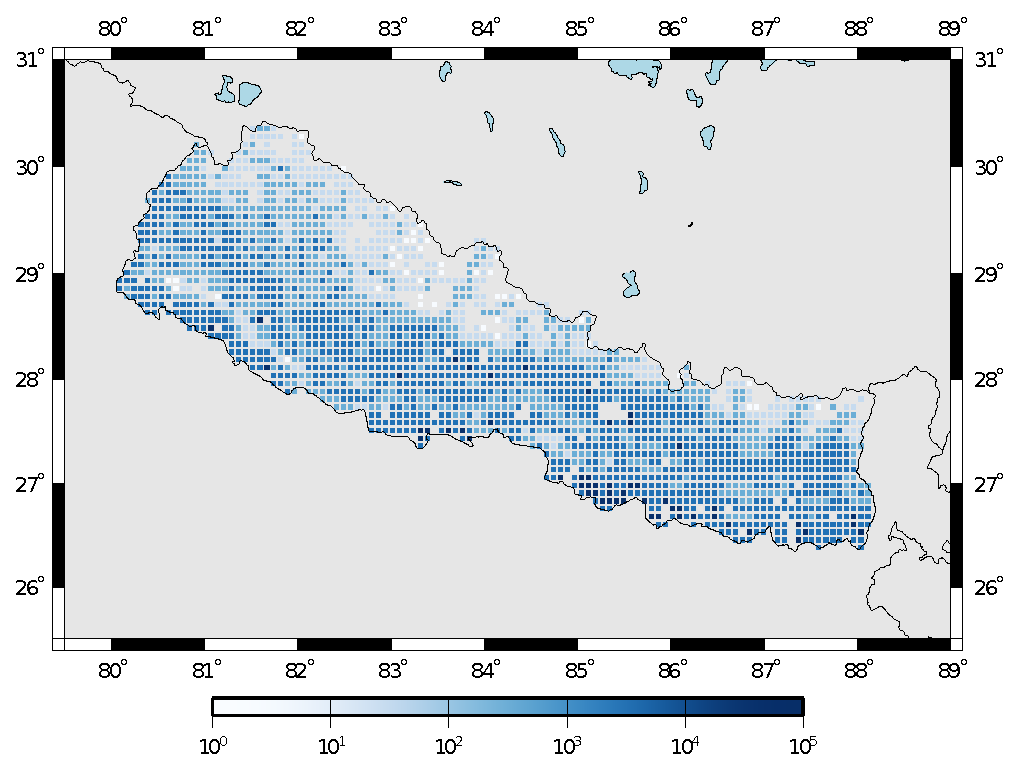
\includegraphics[width=12cm,height=8cm]{./figures/risk/NepalExposure.eps}
\caption{Distribution of number of buildings in Nepal.}
\label{fig:expNepal}
\end{figure}

The building portfolio was organised into four classes for the rural areas (adobe, dressed stone, unreinforced fired brick, wooden frames), and five classes for the urban areas (the aforementioned typologies, in addition to reinforced concrete buildings). For each one of these building typologies, \glspl{vulnerability function} and \glspl{fragility function} were collected from the literature. These input models are only for demonstrative purposes and for further information about the building characteristics of Nepal, users are advised to contact the National Society for Earthquake Technology of Nepal (NSET - \href{http://www.nset.org.np/}{http:www.nset.org.np/}).

This section includes instructions not only on how to run the risk calculations, but also on how to produce the necessary hazard input. Thus, each demo comprises the configuration file, exposure model and fragility/vulnerability models fundamental for the risk calculations, but also a configuration file and associated input models to produce the hazard input.

\section{Scenario Risk demo}
A rupture of magnitude 7 Mw in the central part of Nepal was considered within this demo. The characteristics of this rupture (geometry, dip, rake, hypocentre,  upper and lower seismogenic depth) have been defined in the \verb+rupture.xml+ file, whist the hazard calculation settings have been established on the \verb+job_haz_ini+ file. In order to calculate the set of ground motion fields due to this rupture, users should navigate to the folder where the demo files are located, and use the following command:

\begin{Verbatim}[frame=single, commandchars=\\\{\}, samepage=true]
user@ubuntu:~\$ openquake --rh job_gmfq.ini
\end{Verbatim}

which will produce the following hazard result:

\begin{Verbatim}[frame=single, commandchars=\\\{\}, samepage=true]
Calculation 10 results:
id | output_type | name
20 | gmf_scenario | gmf_scenario
\end{Verbatim}

Then, this hazard input can be used for the risk calculations using the following command:

\begin{Verbatim}[frame=single, commandchars=\\\{\}, samepage=true]
user@ubuntu:~\$ openquake --rr job_risk.ini --hazard-output-id 20
\end{Verbatim}

leading to the following results:

\begin{Verbatim}[frame=single, commandchars=\\\{\}, samepage=true]
Calculation 11 results:
id | output_type | name
21 | aggregate_loss | Aggregate Loss type=structural
22 | loss_map | loss maps. type=structural
\end{Verbatim}

\section{Scenario Damage demo}
The same rupture described in the Scenario Risk demo was used for this demo. The workflow to produce the set of ground motion fields described in the previous section is also valid herein. Then, to run the Scenario Damage demo, users should move to the folder where the required files have been placed and employ following command:

\begin{Verbatim}[frame=single, commandchars=\\\{\}, samepage=true]
user@ubuntu:~\$ openquake --rr job_damage.ini --hazard-output-id 20
\end{Verbatim}

and the following outputs will be produced:

\begin{Verbatim}[frame=single, commandchars=\\\{\}, samepage=true]
Calculation 12 results:
id | output_type | name
23 | collapse_map | Collapse Map per Asset
24 | dmg_dist_per_asset | Damage Distribution per Asset
25 | dmg_dist_per_taxonomy | Damage Distribution per Taxonomy
26 | dmg_dist_total | Damage Distribution Total
\end{Verbatim}

\section{Classical PSHA-based Risk demo}
\label{sec:classical_risk_demo}
The seismic source model developed within the Global Seismic Hazard Assessment Program (GSHAP) was used with the \cite{chiou2008} ground motion prediction equation to produce the hazard input for this demo. No uncertainties are considered in the seismic source model and since only one GMPE is being considered, there will be only one possible path in the logic tree. Therefore, only one set seismic hazard curves will be produced. To do so, the following command needs to be employed:

\begin{Verbatim}[frame=single, commandchars=\\\{\}, samepage=true]
user@ubuntu:~\$ openquake --rh job_hazard.ini
\end{Verbatim}

which will produce the following hazard output:

\begin{Verbatim}[frame=single, commandchars=\\\{\}, samepage=true]
Calculation 13 results:
id | output_type | name
27 | hazard_curve | hc-rlz-70
\end{Verbatim}

In this demo, loss exceedance curves for each asset and two probabilistic loss maps (for probabilities of exceedance of 1\% and 10\%) are produced. The following command launches these risk calculations:

\begin{Verbatim}[frame=single, commandchars=\\\{\}, samepage=true]
user@ubuntu:~\$ openquake --rr job_risk.ini --hazard-output-id 27
\end{Verbatim}

and the following outputs are expected:

\begin{Verbatim}[frame=single, commandchars=\\\{\}, samepage=true]
Calculation 14 results:
id | output_type | name
28 | loss_curve | loss curves. type=structural, hazard=27
29 | loss_map | loss maps. type=structural poe=0.1, hazard=27
30 | loss_map | loss maps. type=structural poe=0.01, hazard=27
\end{Verbatim}

\section{Probabilistic Event-based demo}
This demo uses the same probabilistic seismic hazard assessment (PSHA) model described in the previous example. However, instead of hazard curves, sets of ground motion fields are required. To trigger the hazard calculations the following command needs to be used:

\begin{Verbatim}[frame=single, commandchars=\\\{\}, samepage=true]
user@ubuntu:~\$ openquake --rh job_hazard.ini
\end{Verbatim}

and the following results are expected:

\begin{Verbatim}[frame=single, commandchars=\\\{\}, samepage=true]
Calculation 15 results:
id | output_type | name
31 | gmf | gmf-rlz-72
32 | ses | ses-coll-rlz-72
\end{Verbatim}

Again, since there is only one branch in the logic tree, only one set of ground motion fields will be used in the risk calculations, which can be launched through the following command:

\begin{Verbatim}[frame=single, commandchars=\\\{\}, samepage=true]
user@ubuntu:~\$ openquake --rr job_risk.ini --hazard-output-id 31
\end{Verbatim}

leading to the following outputs:

\begin{Verbatim}[frame=single, commandchars=\\\{\}, samepage=true]
Calculation 16 results:
id | output_type | name
28 | loss_curve | loss curves. type=structural, hazard=31
29 | loss_map | loss maps. type=structural poe=0.1, hazard=31
30 | loss_map | loss maps. type=structural poe=0.01, hazard=31
36 | agg_loss_curve | Aggregated curve type=structural, hazard=31
\end{Verbatim}

\section{Retrofitting Benefit/cost ratio demo}
The loss exceedance curves used within this demo are produced using the Classical PSHA-based Risk calculator. Thus, the process to produce the seismic hazard curves described in the respective section (\ref{sec:classical_risk_demo}) can be employed here. Then, the risk calculations can be initiated using the following command:

\begin{Verbatim}[frame=single, commandchars=\\\{\}, samepage=true]
user@ubuntu:~\$ openquake --rr job_bcr.ini --hazard-output-id 27
\end{Verbatim}

which should produce the following output:

\begin{Verbatim}[frame=single, commandchars=\\\{\}, samepage=true]
Calculation 17 results:
id | output_type | name
37 | bcr_distribution | BCR Distribution for hazard 27
\end{Verbatim}